%=========================================================================
% Start of first day's activities
%=========================================================================
\preClass{Riemann Sums}

\begin{problem}
  \item Determine the value of the integral
  \begin{eqnarray*}
    \int^3_1 f(x) ~ dx,
  \end{eqnarray*}
  where the graph of the function, $f(x)$, is given below.

   \begin{tikzpicture}[scale=2.5]
     \draw[step=1,loosely dotted,line width=1] (-1,-1) grid (4,4);
     \draw[line width=2.2,->] (-1,0) -- (4,0);
     \draw[line width=2.2,->] (0,-1) -- (0,4);
     \begin{scope}
       \clip (0,0) rectangle (2,2);
       \draw[red] (1,0) circle(1.0);
     \end{scope}
     \draw[red] (2,0) -- (3,3);
     \node[left] at (-0.2,3.5) {$f$};
     \node[below] at (3.5,-0.2) {$x$};
     \foreach \x in {-1,1,2,3,4}
        \draw (\x,1pt) -- (\x,-3pt) node[anchor=north east] {\x};
     \foreach \y in {-1,1,2,3,4}
         \draw (1pt,\y) -- (-3pt,\y) node[anchor=north east] {\y};
    \end{tikzpicture}

  \clearpage

  \item Approximate the integral
  \begin{eqnarray*}
    \int^3_1 \ln(x) ~ dx
  \end{eqnarray*}
  using a Riemann sum with 3 rectangles of equal width.

  \clearpage

\end{problem}


\actTitle{Riemann Sums}

\begin{problem}
\item A 5m rod has a charge density given by
  \begin{eqnarray*}
    \lambda_q & = & 5x~\frac{\mathrm{C}}{\mathrm{m}},
  \end{eqnarray*}
  where $x$ is between 0m and 5m.
  \begin{subproblem}
  \item Make a rough sketch of the rod.
    \vspace{4em}
  \item Divide the rod into 5 equal parts, and determine the length of
    each part, and the coordinates for the endpoints.
    \vfill
  \item Determine the charge density at the left endpoint of each part
    of the rod.
    \vfill
    \clearpage
  \item Determine an estimate for the total charge of each part
    assuming that the charge density is roughly constant over each
    part.
    \vfill
    \vfill
  \item Determine an estimate for the total charge in the rod.
    \vfill
    \vfill
  \item Make a sketch of the charge density function, and indicate the geometric relationship between the density and the total charge.
      \vfill
  \end{subproblem}
\end{problem}

\postClass

\begin{problem}
\item Briefly state two ideas from today's class.
  \begin{itemize}
  \item
  \item
  \end{itemize}
\item
  \begin{subproblem}
    \item
  \end{subproblem}
\end{problem}



%=========================================================================
% Start of second day's activities
%=========================================================================
\preClass{Integrals}

\begin{problem}
  \item Determine the value of the following integrals.
    \begin{subproblem}
    \item $\int^5_0 2x ~ dx$
      \vfill
    \item $\int^5_0 2x^2 ~ dx$
      \vfill
    \item $\int^5_0 2x^2 - 2x ~ dx$
      \vfill
    \end{subproblem}
\end{problem}


\actTitle{Integrals}

\begin{problem}
\item A thin rod has a charge density given by
  \begin{eqnarray*}
    \lambda_q & = & x e^{-x^2}~\frac{\mathrm{C}}{\mathrm{m}},
  \end{eqnarray*}
  where $x$ is between 1m and 5m.
  \begin{subproblem}
  \item Make a rough sketch of the rod.
    \vspace{4em}
  \item Divide the rod into 5 equal parts, and determine the length of
    each part, and the coordinates for the endpoints.
    \vfill
  \item Determine the formula for the charge density on the left
    endpoint of each part from above.
    \vfill
  \item Use the charge densities above to approximate the total charge in the rod.
    \vfill
    \clearpage
 \item Make a rough sketch of the rod.
      \vspace{3em}
\item Divide the rod into $n$ equal parts, and determine the length of
      each part, and the coordinates for the endpoints.
      \vfill
  \item Determine the sum using sigma notation for the estimate of the
    total charge in the rod.
    \vfill
  \item Express the limit of the sum as an integral.
    \vfill
  \item Determine the amount of charge in the rod.
    \vfill
  \item Make a sketch of the charge density function, and indicate the geometric relationship between the density and the total charge.
    \vfill
  \end{subproblem}
\end{problem}

\postClass

\begin{problem}
\item Briefly state two ideas from today's class.
  \begin{itemize}
  \item
  \item
  \end{itemize}
\item
  \begin{subproblem}
    \item
  \end{subproblem}
\end{problem}


%=========================================================================
% Second Day of U-Substitution
%=========================================================================
\preClass{u-Substitution}

\begin{problem}
\item Determine the values of each of the following integrals.
  \begin{subproblem}
  \item $\int^{10}_1 \frac{1}{1+x^2} ~ dx$
    \vfill
  \item $\int^{10}_1 \frac{x}{1+x^2} ~ dx$
    \vfill
  \item $\int^{10}_1 \frac{e^x}{1+e^{x}} ~ dx$
    \vfill
  \end{subproblem}
\end{problem}


\actTitle{Calculating Total Charge}
\begin{problem}
\item A long, thin rod has a charge distribution, and the length of the rod is
  2m. The left endpoint is $x=0$m, and the right endpoint is
  $x=2$m. Determine the total charge in the rod for the following
  charge densities.
  \begin{subproblem}
    \item $\lambda_q = \frac{e^x}{1+e^{2x}}$ C/m
      \vfill
    \item $\lambda_q = x\sin\lp 1+x^2\rp$ C/m
      \vfill
  \end{subproblem}
  \clearpage
  \item The function $f$ is defined by
  \begin{eqnarray*}
    h(x) & = & \sin(x).
  \end{eqnarray*}
  The function $g$ satisfies $g(0)=0$ and $g(1)=\frac{\pi}{2}$.
  Determine the value of the integral
  \begin{eqnarray*}
    \int^1_0 h(g(x)) g'(x) ~ dx.
  \end{eqnarray*}
  \vfill
\end{problem}


\postClass

\begin{problem}
\item Briefly state two ideas from today's class.
  \begin{itemize}
  \item
  \item
  \end{itemize}
\item
  \begin{subproblem}
    \item
  \end{subproblem}
\end{problem}


%=========================================================================
% First day of int. by parts
%=========================================================================
\preClass{Integraton}

\begin{problem}
  \item We examine the product rule.
  \begin{subproblem}
    \item   State the product rule for the function below:
  \begin{eqnarray*}
    \lefteqn{\frac{d}{dt} \lp f(t) g(t) \rp  ~ = } \hspace{20em} \\
    & &
  \end{eqnarray*}
  \item Use the product rule to expand the derivative of $f$ in terms of
      $g$ and $g'$:
      \begin{eqnarray*}
        \frac{d}{dt} f(t) & = &  \frac{d}{dt} \lp g(t) e^t \rp
      \end{eqnarray*}
      \vfill
  \item   Solve the previous equation for $g(t) \cdot e^t$.
  \vfill
\end{subproblem}
\end{problem}



\actTitle{Integration by Parts}
\begin{problem}
\item A rod has a charge distribution, and the length of the rod is
  3m. The left endpoint is $x=0$m, and the right endpoint is
  $x=3$m. Determine the total charge in the rod for the following
  charge densities.
  \begin{subproblem}
    \item $\lambda_q = xe^{4x}$ C/m
      \vfill
    \item $\lambda_q = 3+x\sin(5x)$ C/m
      \vfill
      \clearpage
    \item $\lambda_q = x^2 e^{2x} $ C/m
      \vfill
  \end{subproblem}
  \item  Determine the value of the integral
  \begin{eqnarray*}
    \int_{x=0}^\infty x e^{-sx} ~ dx,
  \end{eqnarray*}
  where $s>0$.
  This integral is a function of a variable. What variable is it a function of?
  \vfill
\end{problem}

\postClass

\begin{problem}
\item Briefly state two ideas from today's class.
  \begin{itemize}
  \item
  \item
  \end{itemize}
\item
  \begin{subproblem}
    \item
  \end{subproblem}
\end{problem}


%=========================================================================
% First day of int. by parts / Day II
%=========================================================================
\preClass{Integraton}

\begin{problem}
\item Determine the values of each of the following integrals.
  \begin{subproblem}
  \item $\int^{3}_1 x e^{-x} ~ dx$
    \vfill
  \item $\int^{3\pi}_1 x^2 e^{2x} ~ dx$
    \vfill
  \end{subproblem}
\end{problem}



\actTitle{Integration by Parts}
\begin{problem}
\item A rod has a charge distribution, and the length of the rod is
  3m. The left endpoint is $x=1$m, and the right endpoint is
  $x=3$m. Determine the total charge in the rod for the following
  charge densities.
  \begin{subproblem}
    \item $\lambda_q = \frac{\ln(x)}{x^2} $ C/m
      \vfill
    \item $\lambda_q = e^{\sqrt{x}}$ C/m
      \vfill
  \end{subproblem}
  \clearpage
  \item  Determine the value of the integral
  \begin{eqnarray*}
    \int_{x=0}^\infty \cos(x) e^{-sx} ~ dx,
  \end{eqnarray*}
  where $s>0$.
  This integral is a function of a variable. What variable is it a function of?
  \vfill
\end{problem}

\postClass

\begin{problem}
\item Briefly state two ideas from today's class.
  \begin{itemize}
  \item
  \item
  \end{itemize}
\item The questions below refer to the integral
\begin{eqnarray*}
  \int^M_0 f'(x) e^{-sx} ~ dx,
\end{eqnarray*}
where $s>0$.
  \begin{subproblem}
    \item Use integration by parts to change the integral into an integral
    that has $f(x)$ and not its derivative.
     \vfill
     \item Simplify the expression by assuming that $f(M)e^{-sM}$ goes to zero as $M\rightarrow\infty$.
     \
  \end{subproblem}
\end{problem}


%=========================================================================
% Trig substitutions
%=========================================================================
\preClass{Integraton}

\begin{problem}
\item For each of the triangles below, determine the length of the
  side with the missing length. Also, determine the sine, cosine, and tangent
  for the angle in the lower right part of the triangle.
  \begin{subproblem}
  \item 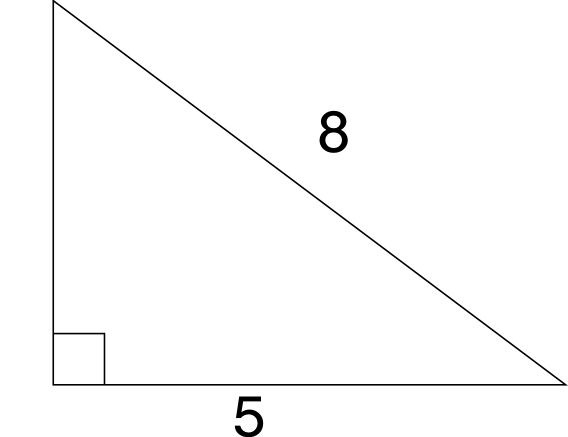
\includegraphics[width=10em]{ink/trigSubs/triangleValuesBottomHyp}
    \vfill
  \item 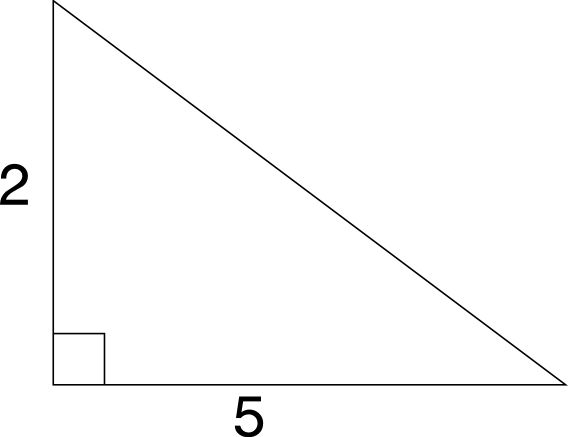
\includegraphics[width=10em]{ink/trigSubs/triangleValuesLeftBottom}
    \vfill
  \item 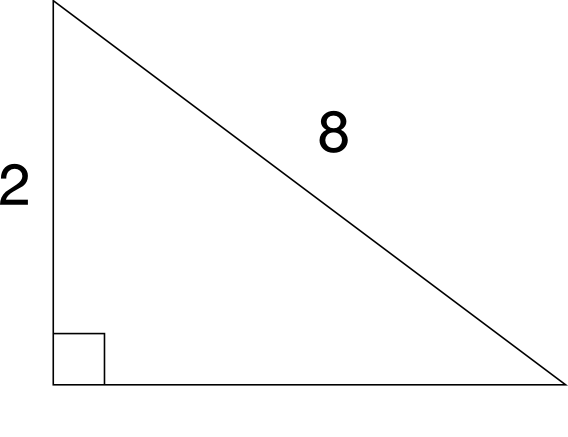
\includegraphics[width=10em]{ink/trigSubs/triangleValuesLeftHyp}
    \vfill
  \end{subproblem}
\end{problem}



\actTitle{Trigonometric Substitution}
\begin{problem}
  \item  A rod of length 2m has a uniform charge density, $\lambda_q$ C/m.
  The center of the rod is placed at the origin and is aligned along the
  $x$-axis.
  \begin{subproblem}
    \item Make a rough sketch of the rod.
         \vspace{5em}
   \item Divide the rod into $n$ equal parts, and determine the length of
         each part, and the coordinates for the endpoints.
         \vspace{2em}
     \item Mark a point 1m above the center of the rod in your picture. Determine the
         electric field due to the charge in one small piece of the rod.
         (Determine the $\vec{i}$ and $\vec{j}$ components separately.)
       \vfill
     \item Add up the components of the electic field to get a sum representing the
      $\vec{i}$ and $\vec{j}$ components of the electic field.
      \vfill
    \clearpage
    \item Determine the integrals that represent the $\vec{i}$ and $\vec{j}$ components of the electic field.
      Determine the values of the integrals and determine the electric field above the center of the rod.
      \vfill
  \end{subproblem}

\end{problem}

\postClass

\begin{problem}
\item Briefly state two ideas from today's class.
  \begin{itemize}
  \item
  \item
  \end{itemize}
  \item A rod has a charge distribution.
    The left endpoint is $x=0$m, and the right endpoint is
    $x=0.5$m. Determine the total charge in the rod for the following
    charge densities.
    \begin{subproblem}
      \item $\lambda_q = \frac{1}{\sqrt{1-x^2}}$ C/m
        \vfill
      \item $\lambda_q = \frac{1}{\sqrt{4-x^2}}$ C/m
        \vfill
    \end{subproblem}
  \item  A rod of length 4m has a uniform charge density, $\lambda_q$ C/m.
    The center of the rod is placed at the origin and is aligned along the
    $x$-axis.
    \begin{subproblem}
      \item Determine the electric field 1m above the center of the rod.
      \item Determine the electric field $l$m above the center of the rod,
        where $l$ is a constant.
      \item Determine the electric field at any point above the rod.
    \end{subproblem}

  \item  A rod of infinite length has a uniform charge density, $\lambda_q$ C/m.
      \begin{subproblem}
        \item Determine the electric field 1m above the rod.
        \item Determine the electric field $l$m above the rod,
          where $l$ is a constant.
        \item Determine the electric field at any point above the rod.
      \end{subproblem}


\end{problem}


%=========================================================================
% Trig substitutions - day 2
%=========================================================================
\preClass{Integraton}

\begin{problem}
\item For each of the triangles below, determine the length of the
  side with the missing length. Also, determine the sine, cosine, and tangent
    for the angle in the lower right part of the triangle.
  \begin{subproblem}
  \item 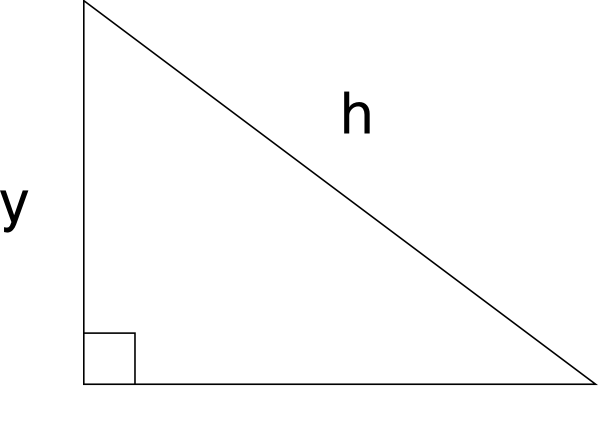
\includegraphics[width=10em]{ink/trigSubs/triangleSymbolsLeftHyp}
    \vfill
  \item 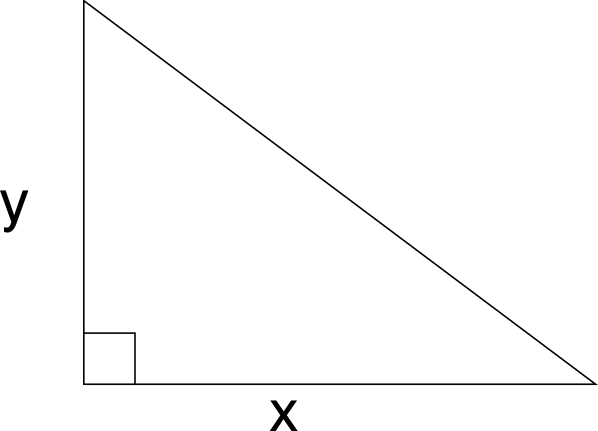
\includegraphics[width=10em]{ink/trigSubs/triangleSymbolsBottomLeft}
    \vfill
  \item 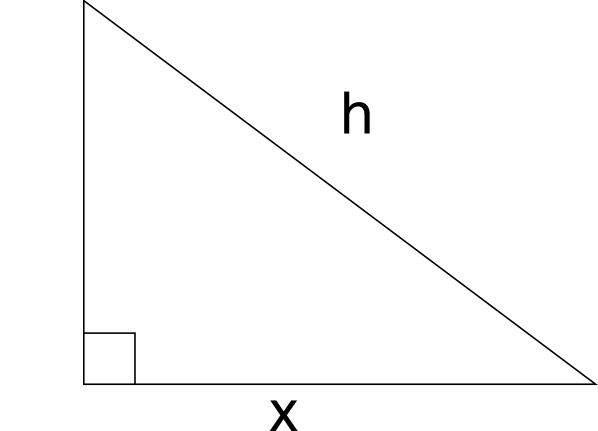
\includegraphics[width=10em]{ink/trigSubs/triangleSymbolsBottomHyp}
    \vfill
  \end{subproblem}
\end{problem}



\actTitle{Trigonometric Substitution}
\begin{problem}
  \item  A rod of length 4m has a uniform charge density, $\lambda_q$ C/m.
  The center of the rod is placed at the origin and is aligned along the
  $x$-axis.
  \begin{subproblem}
    \item Make a rough sketch of the rod.
         \vspace{5em}
   \item Divide the rod into $n$ equal parts, and determine the length of
         each part, and the coordinates for the endpoints.
         \vspace{2em}
     \item Mark a point 3m above the \textbf{right end} of the rod in your picture. Determine the
         electric field due to the charge in one small piece of the rod.
         (Determine the $\vec{i}$ and $\vec{j}$ components separately.)
       \vfill
     \item Add up the components of the electic field to get a sum representing the
      $\vec{i}$ and $\vec{j}$ components of the electic field.
      \vfill
    \clearpage
    \item Determine the integrals that represent the $\vec{i}$ and $\vec{j}$ components of the electic field at the point.
      Determine the values of the integrals and determine the electric field above the center of the rod.
      \vfill
  \end{subproblem}

\clearpage

\item A rod has a charge distribution, and the length of the rod is
  3m. The left endpoint is $x=0$m, and the right endpoint is
  $x=3$m. Determine the total charge in the rod for the following
  charge densities.
  \begin{subproblem}
    \item $\lambda_q = \frac{x}{\sqrt{9-x^2}}$ C/m
      \vfill
    \item $\lambda_q = \frac{x^2}{\sqrt{x^2-9}}$ C/m
      \vfill
  \end{subproblem}
\end{problem}

\postClass

\begin{problem}
\item Briefly state two ideas from today's class.
  \begin{itemize}
  \item
  \item
  \end{itemize}
\item A rod of length $l$ has a uniform charge density, $\lambda_q$ C/m,
    and the right side of the rod is located at the origin.
    \begin{subproblem}
      \item Determine the electric field $y$m above the right side of the rod,
        where $y$ is a constant.
      \item Determine what happens as the length $l$ gets extremely long.
        Does the electric field approach a particular value?
    \end{subproblem}
\item A rod has a charge distribution, and the length of the rod is
  2m. The left endpoint is $x=1$m, and the right endpoint is
  $x=1$m. Determine the total charge in the rod for the following
  charge densities.
  \begin{subproblem}
    \item $\lambda_q = \frac{x}{\sqrt{1+x^2}}$ C/m
      \vfill
    \item $\lambda_q = \frac{x^3}{\sqrt{4+x^2}}$ C/m
      \vfill
  \end{subproblem}
\end{problem}


%=========================================================================
% E-Field for a ring
%=========================================================================
\preClass{Arc-length of a circle.}

\begin{problem}
\item A person moves around a circle of radius 10m. Answer each of the questions below.
  \begin{subproblem}
  \item If the person moves around the whole circle how far has she traveled?
    \vfill
  \item If the person moves half way around the circle, through an angle of $\pi$, how far has she traveled?
    \vfill
  \item If the person moves around the circle through an angle of $\frac{\pi}{4}$ how far has she traveled?
    \vfill
  \item In general, if a person moves around a circle of radius $r$ through an angle $\theta$ how far has she traveled?
      \vfill
  \end{subproblem}
\end{problem}



\actTitle{Electric Field in Three Dimensions}
\begin{problem}
  \item  A thin, circular piece of metal has a uniform charge. The center of the circle is the origin,
        and it lies in the $x-y$ plane. The goal is to determine the electric field at a point above the
        center of the circle. The ring has a uniform charge, $\lambda_q$ C/m. \\
        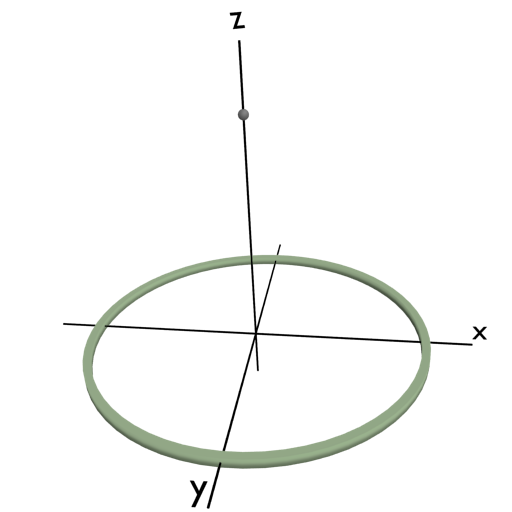
\includegraphics[width=15em]{blender/ringCharge}
  \begin{subproblem}
    \item Which direction do you think the electric field will point at the point above the circle? Why?
             \vspace{3em}
   \item The idea is to divide the ring into small pieces. Determine the charge in a small piece of the ring
       assuming that the length of the small piece is $\triangle s$. \\
           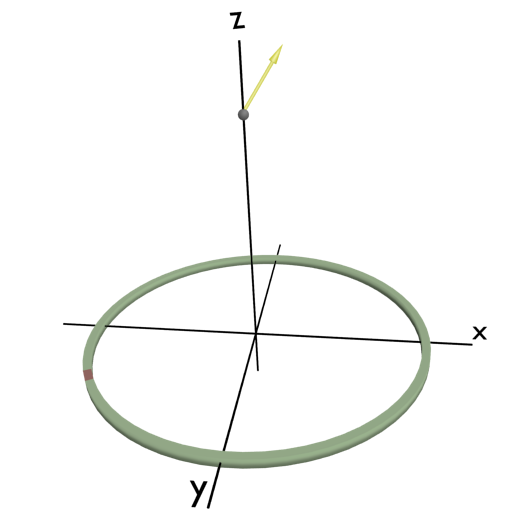
\includegraphics[width=10em]{blender/ringCharge-deltaE}

    \item If the point above the ring is a distance $l$ m over the origin and the radius of the circle is $R$,
      determine the magnitude of the electric field for the small piece. \\
        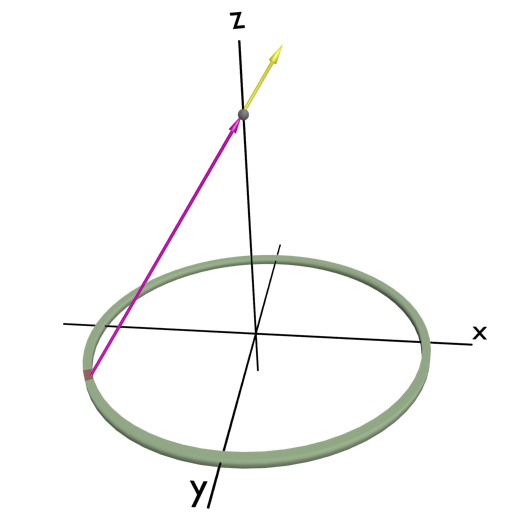
\includegraphics[width=10em]{blender/ringCharge-distance}

    \clearpage

     \item The electric field has three dimensions, components in the $\vec{i}$, $\vec{j}$, and $\vec{k}$ directions.
        The point above the ring is $l$ m above the center of the ring.
       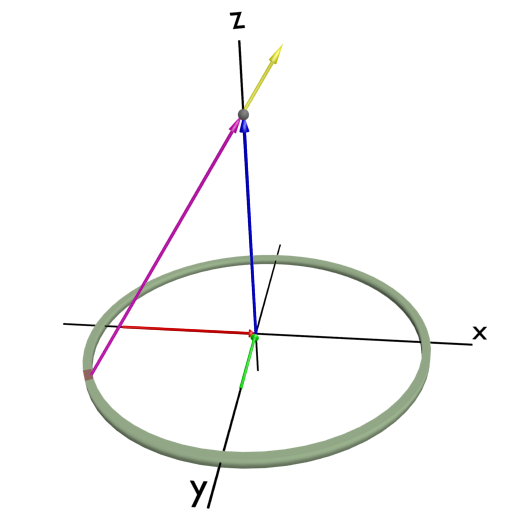
\includegraphics[width=15em]{blender/ringCharge-components}
       \begin{enumerate}
         \item Determine the component of $\triangle \vec{E}$ in the $z$-direction. (Hint: draw a side view of the triangle.)
         \vfill
         \item Determine the component of $\triangle \vec{E}$ pointing in the direction from the small piece towards the origin in the $x-y$ plane.
         \vfill
         \item Determine the component of $\triangle \vec{E}$ in the $x$-direction in terms of $\theta$.
         \vfill
         \item Determine the component of $\triangle \vec{E}$ in the $y$-direction in terms of $\theta$.
         \vfill
       \end{enumerate}
       \clearpage
     \item Determine the length of the small piece of charge in terms of $r$ and $\triangle\theta$.
         \vspace{2em}
     \item Add up the components of the electic field to get a sum representing the
      $\vec{\imath}$, $\vec{\jmath}$, and $\vec{k}$ components of the electic field.
      \vfill
    \item  Determine the Riemann sum that approximates the $\vec{\imath}$, $\vec{\jmath}$, and $\vec{k}$ components of the electic field at the point.
      \vspace{4em}
    \item Determine the integrals that represent the $\vec{\imath}$, $\vec{\jmath}$, and $\vec{k}$ components of the electic field at the point.
      Determine the values of the integrals and determine the electric field above the center of the rod.
      \vfill
      \vfill
      \vfill
  \end{subproblem}

\end{problem}

\postClass

\begin{problem}
\item Briefly state two ideas from today's class.
  \begin{itemize}
  \item
  \item
  \end{itemize}
\end{problem}

%=========================================================================
% E-Field for a plate
%=========================================================================
\preClass{Electric field for a ring}

\begin{problem}
\item Use the results from the previous activity.
  \begin{subproblem}
  \item What is the electric field for a point $l$ meters above the center of a thin ring of radius $r$ above the ring?
    The charge density on the ring is a constant, $\lambda_q$ C/m.
    \vfill
  \item What is the area of a circle of radius $r$?
    \vfill
  \item What is the area of a circle of radius $r+\triangle r$?
      \vfill
  \item What is the area between a circle of radius $r$ and a circle of radius $r+\triangle r$?
    \sideNote{Foil out the value and simplify it as much as possible.}
      \vfill
  \end{subproblem}
\end{problem}



\actTitle{Electric Field Over a Circular Plate}
\begin{problem}
  \item The goal is to derive the function that represents the electric field over the center of
    a thin circular plate with radius $R$ and a constant charge density $\sigma_q$ C/m\textsuperscript{2}.
    Refer to the previous day's activities and repeat the steps on your own.
  \begin{subproblem}
    \item Draw a picture of the plate with a point $l$ meters above the center of the plate.
      \vfill
   \item Divide the plate into thin rings each with width $\triangle r$.  (Redraw the picture.)
      \vfill
   \item Determine the electric field for one of the thin rings.  (Redraw the picture.)
       \vfill

    \clearpage

   \item Determine the domain of the function representing the electric field, $\triangle \vec{E}$
      for the small ring. (What variable is changing for the different rings?)
      \vspace{2em}

    \item Determine the Riemann sum for the electric field at the point above the ring.
      \vfill

    \item Determine the integral and solve the intregal that represents the electric field at the point above the ring.
      \vfill
      \vfill
      \vfill

    \clearpage

    \item Is the result consistent with the physical situation? Does it make sense?
       \vfill

     \item What happens as the radius of the disk increases?
        \vfill

      \item What happens as the distance above the disk increases?
       \vfill

  \end{subproblem}
\end{problem}

\postClass

\begin{problem}
\item Briefly state two ideas from today's class.
  \begin{itemize}
  \item
  \item
  \end{itemize}
\end{problem}

%=========================================================================
% Start of Volumes of Revolution
%=========================================================================
\preClass{Volumes of Revolution}

\begin{problem}
\item Determine the value of the integral
  \begin{eqnarray*}
    \int^h_0 \pi \left (R-\frac{R}{h} x\right)^2 ~ dx,
  \end{eqnarray*}
  where $h$ and $R$ are constants.
  \vfill

\item What is the volume of a right circular cylinder resting on its
  edge that has a radius of $R$ and a height $h$?

  \vfill

\item What is the volume of two cylinders resting on their edge
  standing next to each other? The first is a right circular cylinder
  that has a radius of $R_1$ and a height $h_1$, and the second is a
  right circular cylinder that has a radius of $R_2$ and a height
  $h_2$.

  \vfill

\end{problem}


\actTitle{Volumes of Revolution}
\begin{problem}
\item Determine the formula for a line that will be revolved
      around the $x$-axis, and the resulting solid will be a right
      circular cone of radius $R$ and height $h$.
  \begin{subproblem}
    \item Make a sketch of the line. (Make an axis and clear mark the
      axes.)
      \vfill

    \item Make a sketch of the resulting solid obtained after
      revolving the line around the $x$ axis.
      \vfill

    \item Determine the integral that represents the volume of the
      cone using washers.
      \vfill

  \end{subproblem}
\end{problem}

\postClass

\begin{problem}
\item Briefly state two ideas from today's class.
  \begin{itemize}
  \item
  \item
  \end{itemize}
\item
  \begin{subproblem}
    \item
  \end{subproblem}
\end{problem}


%=========================================================================
% Start of Volumes of Revolution
%=========================================================================
\preClass{Volumes of Revolution}

\begin{problem}
\item Determine the value of the integral
  \begin{eqnarray*}
    \int^R_0 2\pi x \left( R-x \right) ~ dx.
  \end{eqnarray*}
  \vfill

\item What is the volume of a right circular cylinder that has a
  radius of $R$ and a height $h$ that is resting on its base?

  \vfill

\item What is the volume of two cylinders stacked on top of one
  another vertically? The first is a right circular cylinder that has a radius of
  $R_1$ and a height $h_1$, and the second is a right circular cylinder that
  has a radius of $R_2$ and a height $h_2$.

  \vfill

\end{problem}


\actTitle{Volumes of Revolution}
\begin{problem}
\item Determine the formula for a line that will be revolved
      around the $y$-axis, and the resulting solid will be a right
      circular cone of radius $R$ and height $h$.
  \begin{subproblem}
    \item Make a sketch of the line. (Make an axis and clear mark the
      axes.)
      \vfill

    \item Make a sketch of the resulting solid obtained after
      revolving the line around the $y$ axis.
      \vfill

    \item Determine the integral that represents the volume of the
      cone using shells.
      \vfill

  \end{subproblem}
\end{problem}

\postClass

\begin{problem}
\item Briefly state two ideas from today's class.
  \begin{itemize}
  \item
  \item
  \end{itemize}
\item
  \begin{subproblem}
    \item
  \end{subproblem}
\end{problem}



%=========================================================================
% Start of Areas of Revolution
%=========================================================================
\preClass{Area of Revolution}

\begin{problem}
\item Determine the area of the sector of a circle shown below in
  terms of
  $\theta$ and $R$. \\
  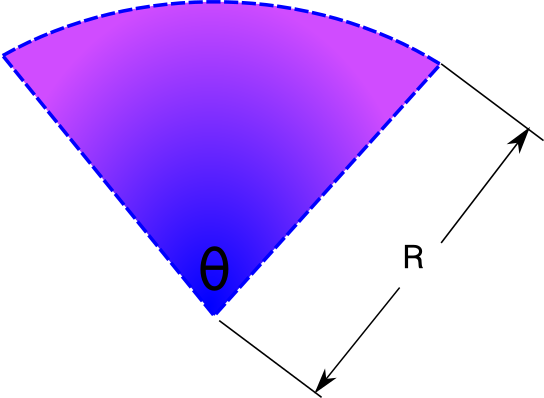
\includegraphics[width=12em]{ink/revolution/sector}

\item Determine the area of the slice of a sector shown below in terms of
  $\theta$, $L_1$, and $L_2$. \\
  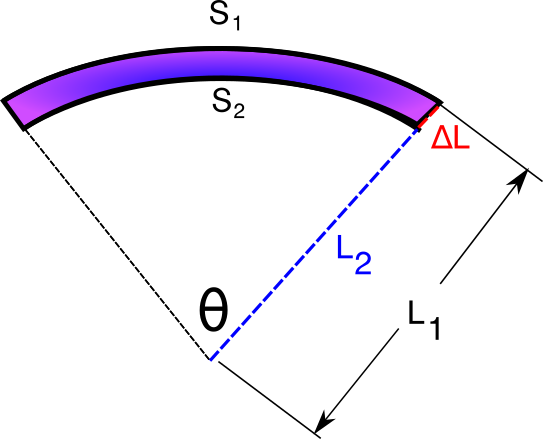
\includegraphics[width=12em]{ink/revolution/sectorDifference}

\item Use the relationship $L_2+\triangle L=L_1$ to express the area
  of the strip in terms of $\theta$, $\triangle L$, and  $L_2$.
  Expand and simplify the result.
  \label{problem:revol:area}
  \vfill

\item Substitute  $L_2\theta=S_2$  into the expression
  for the area in part \ref{problem:revol:area}.

  \vfill

\item Show that ${S_1-S_2}= \triangle L \theta$.

  \vfill


\item Substitute the expression found for $\triangle L \theta$ in the
  expression for the area. Simplify your result, and you should have a
  formula for the area of the strip only in terms of $S_1$, $S_2$, and
  $\triangle L$.

  \vfill

  \sideNote{Hint: $\triangle L^2\theta = \triangle L \cdot \triangle L \theta$}


\end{problem}


\actTitle{Area of Revolution}
\begin{problem}
\item Determine the formula for a line that will be revolved
      around the $x$-axis, and the resulting solid will be a right
      circular cone of radius $R$ and height $h$.
  \begin{subproblem}
    \item Make a sketch of the line. (Make an axis and clear mark the
      axes.)
      \vfill

    \item Make a sketch of the resulting solid obtained after
      revolving the line around the $y$ axis.
      \vfill

    \item Determine the integral that represents the area of the cone.
      \vfill

  \end{subproblem}
\end{problem}

\postClass

\begin{problem}
\item Briefly state two ideas from today's class.
  \begin{itemize}
  \item
  \item
  \end{itemize}
\item
  \begin{subproblem}
    \item
  \end{subproblem}
\end{problem}


%=========================================================================
% Start of partial fractions
%=========================================================================
\preClass{Rational Functions}

\begin{problem}
\item Express each function below as a single fraction. That is bring
  the two parts together over a common denominator and simplify the
  result.
  \begin{subproblem}
  \item $\frac{1}{x+3} + \frac{1}{x+2}$
    \vfill
  \item $\frac{1}{x+3} + \frac{3}{x-2}$
    \vfill
  \item $\frac{1}{x+3} + \frac{4}{x-3}$
    \vfill
  \end{subproblem}
\end{problem}


\actTitle{Partial Fractions}
\begin{problem}
\item Determine the common denominator for each of the expressions below.
  \begin{subproblem}
    \item $\frac{1}{x} + \frac{1}{x-3}$ \\
      Common Denominator: \framebox(250,50){~}
      \vfill
    \item $\frac{8}{x+7} + \frac{20}{x+50}$ \\
      Common Denominator: \framebox(250,50){~}
      \vfill
    \item $\frac{8,250}{x+7} + \frac{x}{x+50}$ \\
      Common Denominator: \framebox(250,50){~}
      \vfill
  \end{subproblem}

  \clearpage

\item For each of the following functions write the general form of
  the partial fraction expansion. The first one is completed as an
  example.
  \begin{subproblem}
    \item $\frac{2x+1}{x^2+2x-8}$ \\
      General Form: \framebox(250,50){$\frac{A}{x+4} + \frac{B}{x-2}$}
      \vfill
    \item $\frac{8x+1}{x^2-x-12}$ \\
      General Form: \framebox(250,50){~}
      \vfill
    \item $\frac{5x-10}{x^2-16}$ \\
      General Form: \framebox(250,50){~}
      \vfill
    \item $\frac{4x+2}{x^2-5x}$ \\
      General Form: \framebox(250,50){~}
      \vfill
  \end{subproblem}

\end{problem}

\postClass

\begin{problem}
\item Briefly state two ideas from today's class.
  \begin{itemize}
  \item
  \item
  \end{itemize}
\item
  \begin{subproblem}
    \item
  \end{subproblem}
\end{problem}


\preClass{Rational Functions}

\begin{problem}
\item Express each function below as a single fraction. That is bring
  the two parts together over a common denominator and simplify the
  result.
  \begin{subproblem}
  \item $\frac{1}{x+2} + \frac{3}{(x+2)^2}$
    \vfill
  \item $\frac{1}{x+3} + \frac{2}{(x+3)^2}$
    \vfill
  \item $\frac{1}{x} + \frac{1}{x^2} + \frac{1}{x^2}$
    \vfill
  \end{subproblem}
\end{problem}

\actTitle{Partial Fractions}
\begin{problem}
\item Determine the common denominator for each of the expressions below.
  \begin{subproblem}
    \item $\frac{1}{x-3} + \frac{1}{x^2-6x+9}$ \\
      Common Denominator: \framebox(250,50){~}
      \vfill
    \item $\frac{8}{x+7} + \frac{20}{x^2+14x+49}$ \\
      Common Denominator: \framebox(250,50){~}
      \vfill
    \item $\frac{8,250}{x+7} + \frac{x}{x^2+14x+49}$ \\
      Common Denominator: \framebox(250,50){~}
      \vfill
  \end{subproblem}

  \clearpage

\item For each of the following functions write the general form of
  the partial fraction expansion. The first one is completed as an
  example.
  \begin{subproblem}
    \item $\frac{2x+1}{x^2+2x-8}$ \\
      General Form: \framebox(250,50){$\frac{A}{x+4} + \frac{B}{x-2}$}
      \vfill
    \item $\frac{8x+1}{x^2-x-12}$ \\
      General Form: \framebox(250,50){~}
      \vfill
    \item $\frac{5x-10}{x^2+8x+16}$ \\
      General Form: \framebox(250,50){~}
      \vfill
    \item $\frac{4x+2}{x^2-10x+25}$ \\
      General Form: \framebox(250,50){~}
      \vfill
  \end{subproblem}

\end{problem}


\postClass

\begin{problem}
\item Briefly state two ideas from today's class.
  \begin{itemize}
  \item
  \item
  \end{itemize}
\item
  \begin{subproblem}
    \item
  \end{subproblem}
\end{problem}


\preClass{Rational Functions}

\begin{problem}
\item For each of the quadratic functions below complete the square to
  express each function in the form
  \begin{eqnarray*}
    f(x) & = & A(x-B)^2 + C.
  \end{eqnarray*}
  \begin{subproblem}
  \item $x^2 - 2x + 2$
    \vfill
  \item $x^2 - 6x + 12$
    \vfill
  \item $2x^2 - 4x + 6$
    \vfill
  \end{subproblem}
\end{problem}

\actTitle{Partial Fractions}
\begin{problem}
\item For each integral below complete the square on the denominator
  and then use $u$-substitution to determine the integral.
  \begin{subproblem}
    \item ${\displaystyle \int}\frac{1}{x^2 - 2x + 2}~dx$ \\
      \vfill
    \item ${\displaystyle\int}\frac{2}{x^2 - 6x + 12}~dx$ \\
      \vfill
    \item ${\displaystyle\int}\frac{1}{x^2 + 8x + 26}~dx$ \\
      \vfill
  \end{subproblem}

  \clearpage

\item Determine the value of the integral
  \begin{eqnarray*}
    \int \frac{1}{x^3+x^2+3\,x-5} ~ dx
  \end{eqnarray*}

  \vfill

\end{problem}


\postClass

\begin{problem}
\item Briefly state two ideas from today's class.
  \begin{itemize}
  \item
  \item
  \end{itemize}
\item
  \begin{subproblem}
    \item
  \end{subproblem}
\end{problem}





%%% Local Variables:
%%% mode: latex
%%% TeX-master: t
%%% End:
